\section{技术架构}
\subsection{基本情况}
课题目标系统是一个web系统,传统的后台是作为可选的部分存在,主要的应用
是前端,算法运行展示等等都不依托于后台,一部分数据的存储是依托于后台,
作为可选的组件,大多数用户需要的数据都在前端利用HTML5中相应的技术存放,
还可以通过另一个可选的组件,即包装这个web系统的桌面程序,存储到本地的
文件数据库中。
      \begin{figure}[!htb]
      	\centering
      	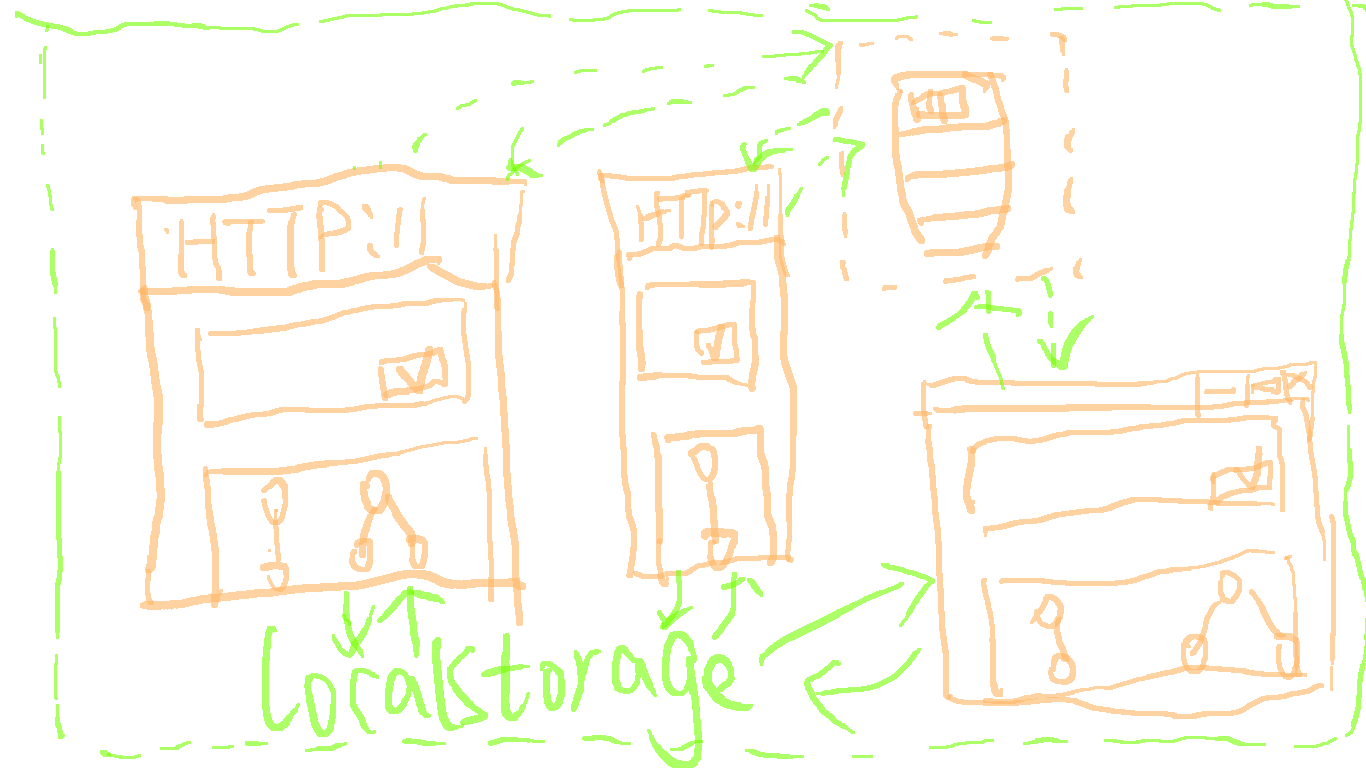
\includegraphics[width=0.7\linewidth]{img/structure.png}
      	\caption{左边桌面浏览器,中间手机浏览器,右边桌面程序,右上可选的服务器,网页可以依托localstorage来存储,也可以借助服务器来存储}
      	\label{fig:structure.png}
      \end{figure}
\subsection{具体架构}
\paragraph{前端逻辑结构} 系统的前端使用了 angular 来组织,利用了
angular中MVVM的架构特点,将前端系统模块化。在项目早期,我们几乎都是用
angular来组织代码,利用angular中的模块,利用angular中的各种成分,功能
构成了最终的系统。但是,angular新版本的出来,让我们意识到这种方式的局
限性,它局限于angular框架,而未来某一天我们可能会换掉这个框架,所以我
们借鉴了angular2的思路,使用了未来的标准模块化的方案。因为是来自于还没
有正式定下来的方案,我们加了一层转换器,也就是使用了一个新的语言
typescript。不过typescript没有增加我们的学习成本,在它上面基本上可以写
javascript,只是多了模块的概念。依靠这个模块和类,我们最终重构了我们的
项目,让现在的项目更容易看懂和测试。angular和typescript共同用于组织代
码,区别代码中的逻辑和视图。
\paragraph{前端界面} 而另一个我们采用的框架bootstrap则是帮我们处理基本
的浏览器兼容问题,并且提供给我们大量可以使用的web组件,便于我们最终创
造一个能在各种设备上面访问的web系统。而且bootstrap并不像其他的UI框架,
具有类似绑架的行为,将我们的系统绑架在他们上面,它本身具有相当开放的开
发方式,便于我们自己定制修改主题,甚至直接写其他的样式,而不用考虑怎么
和bootstrap进行配合。最重要的还有一块动画的部分,我们使用了D3作为一个
重要的展示类库。实际中,D3的帮助还显得不是很大,但是它确实在呈现各类图
标的时候,表现了它的能力。而作为候选,我们还可能直接操作canvas来进行,
如果后期需要更复杂的动画的情况下。D3允许我们通过操作数据,而它负责展示
动画,换句话说,只要我们改变了数据,就会产生相应的动画,其设计的思想和
我们在设计动画的时候,使用的思路是比较类似的。而且D3并不是自己负责给你
安排数据的展现方式,而是你可以设定数据进入移除更新的时候,分别需要采取
的动画形式。也就是说,D3只是帮助我们处理判断前后的数据有哪些不同,从而
应用不同的动画。不过,D3其实也帮助我们实现了很多常见的布局,比如可以很
方便用D3来写一些树状图、韦恩图等等,根据数据的结构,我们可以选择一个合
适的图来表达。
\paragraph{数据存储} 对于一部分的数据存储的需求,具体来说就是将用户输
入的文法进行存储、将生成的步骤序列进行存储、将生成的解析器进行存储等等
这部分需求,我们通过web中存储的API,存储在了浏览器中,从而,用户可以方
便获取这些数据,以便于用户不断重复操作来研究学习。如果用户希望可以把这
些数据存储到服务器中,我们也提供了一个可选的后端,通过后端,用户可以将
数据存储起来,方便自己在各个设备中都可以访问到这些数据。
\paragraph{本地应用}我们还采用了一个名为electron的框架,用于将web程序
封装成本地程序,这个组件可以用在用户没有合适的浏览器可以访问的情况下,
或者用户想要用有更好的浏览体验的时候,可以使用这个组件。通过electron,
我们可以生成不同平台的本地程序提供给用户使用。基于这个组件,我们还可以
拓展这个系统的功能,但是这部分扩展暂时不在计划之内,这里只是说明了一下
它可以做更多web平台可能目前无法做到的事情。
\paragraph{手机扩展}因为采用了angular,所以还有一个可能的扩展是,可以
通过ionic等框架,将应用延伸到手机端,而不需要写额外的代码。这其实有一
个前提,就是设计界面的时候考虑到手机屏幕的问题 ,而我们的界面目前还没
有考虑多少手机操作的问题,这部分内容也属于这个课题目标之外的设想。
\paragraph{后台及前后台交互} 一个可选的后台实际上是由express编写的,处
理一些简单的请求,将对应的数据存储到一个服务器端的文件数据库中,这部分
内容很简单,可以根据更具体的需求进行定制,目前我们只是预想了这部分需求,
并没有更实质性的计划。也就是说,后台的语言并没有局限在某种特定的语言,
也没有局限在特定的框架上面。但是已经考虑到这种想法,所以前台也会避免使
用一些会有冲突的解决方案。
